\documentclass[10pt,letterpaper,twocolumn]{article}
\usepackage[utf8]{inputenc}
\usepackage[spanish]{babel}
\usepackage{listings}
\usepackage[usenames,dvipsnames]{color}
\usepackage{amsmath}
\usepackage{calc}
\usepackage{verbatim}
\usepackage{hyperref}
\usepackage{color}
\usepackage{geometry}
\usepackage[pdftex]{graphicx}
\usepackage{pgfplots}
\usepackage{array}

%Poner la página en landscape
\geometry{verbose,landscape,letterpaper,tmargin=1.5cm,bmargin=2cm,lmargin=1.6cm,rmargin=1.6cm}

\newcommand{\source}[1]{
  \verbatiminput{#1}
  \dotfill
}
\setlength{\columnsep}{0.25in}
\setlength{\columnseprule}{1px}


\begin{document}


\title{Manual de algoritmos para maratones de programación}
\author{Just Code It.}
\date{6 de septiembre de 2014}
\maketitle

\tableofcontents

\section{Plantilla}
  \source{./src/template.cpp}

 \section{Cosas para tener en cuenta}
  \begin{itemize}
    \item Si la respuesta de un problema es un número de punto flotante redondeado y está dando $Wrong Answer$, ensayar
             sumarle un épsilon a la respuesta, es decir, sumarle EPS (siendo EPS por lo general 1e-9).
    \item Recordar que para redondear un número de punto flotante se debe usar el parámetro $\%.xf$ (donde x es la cantidad de cifras)
             en la función $printf$.
    \item En problemas que se trabajen números de punto flotante y enteros a la vez, es recomendable mutiplicar por 1.0 cuando
             se estén haciendo operaciones con ambos tipos de datos. Con esto se evitarán problemas de conversión.
  \end{itemize}

\section{Grafos}

  \subsection{BFS}
    Algoritmo de recorrido de grafos en anchura que empieza desde una fuente $s$ y visita todos los nodos alcanzables desde $s$.\\
    El BFS también halla la distancia más corta entre $s$ y los demás nodos si las aristas tienen todas peso 1.\\
    Complejidad: $O(n+m)$ donde $n$ es el número de nodos y $m$ es el número de aristas.\\
    \source{./src/bfs.cpp}

  \subsection{DFS}
    Algoritmo de recorrido de grafos en profundidad que empieza visita todos los nodos del grafo.\\
    El algoritmo puede ser modificado para que retorne información de los nodos según la necesidad del problema.\\
    El grafo tiene un ciclo $\leftrightarrow$ si en algún momento se llega a un nodo marcado como gris.\\
    Complejidad: $O(n+m)$ donde $n$ es el número de nodos y $m$ es el número de aristas.\\
    \source{./src/dfs.cpp}

  \subsection{Ordenamiento topológico}
    Dado un grafo no cíclico y dirigido (DAG), ordena los nodos linealmente de tal forma que si existe una arista entre los nodos $u$ y $v$ entonces $u$ aparece antes que $v$ en el ordenamiento.\\
    Este ordenamiento se puede ver como una forma de poner todos los nodos en una línea recta y que las aristas vayan todas de izquierda a derecha.\\
    Complejidad: $O(n+m)$ donde $n$ es el número de nodos y $m$ es el número de aristas.
    \source{./src/ordenamiento_topologico.cpp}

  \subsection{Componentes fuertemente conexas}
    Dado un grafo dirigido, calcula la componente fuertemente conexa (SCC) a la que pertenece cada nodo.\\
    Para cada pareja de nodos $u, v$ que pertenecen a una misma SCC se cumple que hay un camino de $u$ a $v$ y de $v$ a $u$.\\
    Si se comprime el grafo dejando como nodos cada una de las componentes se quedará con un DAG.\\
    \subsubsection{Kosaraju's algorithm}
      Complejidad: $O(n+m)$ donde $n$ es el número de nodos y $m$ es el número de aristas.\\
      \source{./src/componentes_conexas.cpp}
    \subsubsection{Tarjan's algorithm}
      \begin{itemize}
        \item $d[i]$ = Tiempo de descubrimiento del nodo i. (Inicializar con -1)
        \item $low[i]$ = Menor tiempo de descubrimiento alcanzable desde el nodo i. (No inicializar)
        \item $scc[i]$ = Componente a la que pertenece el nodo i. (No inicializar)
        \item $s$ = Pila usada por el algoritmo (Inicializar vacía)
        \item $stacked[i]$ = true si el nodo i está en la pila. (Inicializar con falso)
        \item $ticks$ = Reloj usado para los tiempos de descubrimiento (Inicializar en 0)
        \item $current_scc$ = id de la componente actual siendo descubierta. (Inicializar en 0)
        \source{./src/tarjan.cpp}
      \end{itemize}

  \subsection{Algoritmo de Dijkstra}
    Dado un grafo con pesos \textbf{no negativos} en las aristas, halla la mínima distancia entre una fuente $s$ y los demás nodos.\\
    Al heap se inserta primero la distancia y luego en nodo al que se llega. Si se quieren modificar los pesos por \verb|long long| o por \verb|double| se debe cambiar en los tipos de dato \verb|dist_node| y \verb|edge|.\\
    Complejidad: $O((n+m) \operatorname{log} n)$ donde $n$ es el número de nodos y $m$ es el número de aristas.\\
    \source{./src/dijkstra.cpp}

  \subsection{Algoritmo de Bellman-Ford}
    Dado un grafo con pesos cualquiera, halla la mínima distancia entre una fuente $s$ y los demás nodos.\\
    Si hay un ciclo de peso negativo en el grafo, el algoritmo lo indica.\\
    Complejidad: $O(n \times m)$ donde $n$ es el número de nodos y $m$ es el número de aristas.\\
    Tener en cuenta que si el nodo es inalcanzable la distancia que resulta en dicho nodo siempre será infinito.\\
    Si el problema es como $Haunted$ $Graveyard$, donde los niños querian salir del cementerio lo más rápido posible (no querian quedarse dando vueltas así fueran ciclos negativos) entonces no deberia poner aristas en el nodo de salida.\\
    \source{./src/bellman_ford.cpp}

  \subsection{Algoritmo de Floyd-Warshall}
    Dado un grafo con pesos cualquiera, halla la mínima distancia entre cualquier para de nodos.\\
    Si este algoritmo es muy lento para el problema ejecutar $n$ veces el algoritmo de Dijkstra o de Bellman-Ford según el caso.\\
    Complejidad: $O(n^3)$ donde $n$ es el número de nodos.\\ \quad \\
    Casos base:
    $\verb|d[i][j]| =
      \begin{cases}
        0       &\text{\quad si } i = j\\
        w_{i,j} &\text{\quad si existe una arista entre $i$ y $j$}\\
        +\infty &\text{\quad en otro caso}
      \end{cases}$ \\

    \quad \\ \textbf{Nota:} Utilizar el tipo de dato apropiado (\verb|int|, \verb|long long|, \verb|double|) para \verb|d| y para $+\infty$ según el problema.

    \source{./src/floyd-warshall.cpp}

    \subsubsection{Clausura transitiva}
    Dado un grafo cualquiera, hallar si existe un camino desde $i$ hasta $j$ para cualquier pareja de nodos $i, j$\\ \quad \\
    Casos base:
    $\verb|d[i][j]| =
      \begin{cases}
        \verb|true |   &\text{\quad si } i = j\\
        \verb|true |   &\text{\quad si existe una arista entre $i$ y $j$}\\
        \verb|false|   &\text{\quad en otro caso}
      \end{cases}$ \\ \quad \\
    Caso recursivo: \verb|d[i][j] = d[i][j] or (d[i][k] and d[k][j]);|

    \subsubsection{Minimax}
    Dado un grafo con pesos, hallar el camino de $i$ hasta $j$ donde la arista más grande del camino sea lo más pequeña posible.\\
    Ejemplos: Que el peaje más caro sea lo más barato posible, que la autopista más larga sea lo más corta posible.\\ \quad \\
    Casos base:
    $\verb|d[i][j]| =
      \begin{cases}
        0         &\text{\quad si } i = j\\
        w_{i,j}   &\text{\quad si existe una arista entre $i$ y $j$}\\
        +\infty   &\text{\quad en otro caso}
      \end{cases}$ \\ \quad \\
    Caso recursivo: \verb|d[i][j] = min( d[i][j], max (d[i][k], d[k][j]) );|

    \subsubsection{Maximin}
    Dado un grafo con pesos, hallar el camino de $i$ hasta $j$ donde la arista más pequeña del camino sea lo más grande posible.\\
    Ejemplos: Que el trayecto menos seguro sea lo más seguro posible, que la autopista de menos carriles tenga la mayor cantidad de carriles.\\ \quad \\
    Casos base:
    $\verb|d[i][j]| =
      \begin{cases}
        +\infty   &\text{\quad si } i = j\\
        w_{i,j}   &\text{\quad si existe una arista entre $i$ y $j$}\\
        -\infty   &\text{\quad en otro caso}
      \end{cases}$ \\ \quad \\
    Caso recursivo: \verb|d[i][j] = max( d[i][j] , min(d[i][k], d[k][j]) )|


  \subsection{Algoritmo de Prim}
  Dado un grafo no dirigido y conexo, retorna el costo del árbol de mínima expansión de ese grafo.\\
  El costo del árbol de mínima expansión también se puede ver como el mínimo costo de las aristas de manera que haya un camino entre cualquier par de nodos.\\
  Complejidad: $O(m \operatorname{log} n)$ donde $n$ es el número de nodos y $m$ es el número de aristas.\\
    \source{./src/prim.cpp}

  \subsection{Algoritmo de Kruskal}
    \subsubsection{Union-Find}
    Union-Find es una estructura de datos para almacenar una colección conjuntos disjuntos (no tienen elementos en común) que cambian dinámicamente.\\
    Identifica en cada conjunto un ``padre'' que es un elemento al azar de ese conjunto y hace que todos los elementos del conjunto ``apunten'' hacia ese padre. \\
    Inicialmente se tiene una colección donde cada elemento es un conjunto unitario.\\
    Complejidad aproximada: $O(m)$ donde $m$ el número total de operaciones de \verb|initialize|, \verb|union| y \verb|join| realizadas.\\
    \source{./src/union-find.cpp}

    \subsubsection{Algoritmo de Kruskal}
    Dado un grafo no dirigido y conexo, retorna el costo del árbol de mínima expansión de ese grafo.\\
    El costo del árbol de mínima expansión también se puede ver como el mínimo costo de las aristas de manera que haya un camino entre cualquier par de nodos.\\
    Utiliza Union-Find para ver rápidamente qué aristas generan ciclos.\\
    Complejidad: $O(m\operatorname{log} n)$ donde $n$ es el número de nodos y $m$ es el número de aristas.\\
    \source{./src/kruskal.cpp}

  \subsection{Algoritmo de máximo flujo}
    Dado un grafo con capacidades enteras, halla el máximo flujo entre una fuente $s$ y un sumidero $t$.\\
    Como el máximo flujo es igual al mínimo corte, halla también el mínimo costo de cortar aristas de manera que $s$ y $t$ queden desconectados.\\
    Si hay varias fuentes o varios sumideros poner una súper-fuente / súper-sumidero que se conecte a las fuentes / sumideros con capacidad infinita.\\
    Si los nodos también tienen capacidad, dividir cada nodo en dos nodos: uno al que lleguen todas las aristas y otro del que salgan todas las aristas y conectarlos con una arista que tenga la capacidad del nodo.\\
    Complejidad: $O(n \cdot m^2)$ donde $n$ es el número de nodos y $m$ es el número de aristas.\\
    \source{./src/maxflow.cpp}
  \subsection{Teorema de Konig}
    \subsubsection{Ejemplo, aplicación Max Flow - Mimimum Vertex Cover - Maximum Matching Size}
    El algoritmo de máximo flujo es equivalente al problema de $Minimum Vertex Cover$ en un grafo bipartito, pero como el Vertex Cover es NP-hard, entonces el teorema de $Konig$ nos dice que el $Minimum Vertex Cover$ es igual al $Maximum Matching Size$, el cual puede ser encontrado por un máximo flujo estándar.\\
    A continuación se presenta un problema para esta aplicación.\\
\rule{12cm}{.1pt}\\
    As an example, one year there were six interns: Stephen Cook, Vinton Cerf, Edmund Clarke, Judea Pearl, Shafi Goldwasser, and Silvio Micali. They were able to self-organize into three teams:
    \begin{itemize}
      \item Stephen Cook, Vinton Cerf, and Edmund Clarke (whose last names all begin with C)
      \item Shafi Goldwasser and Silvio Micali (whose first names begin with S)
      \item Judea Pearl (not an interesting group, but everyone's first name in this group starts with J)
    \end{itemize}
As a historical note, the company was eventually shut down due to a rather strange (and illegal) hiring practice---they refused to hire any interns whose last names began with the letter S, T, U, V, W, X, Y, or Z. (First names were not subject to such a whim, which was fortunate for our friend Vinton Cerf.)\\
\textbf{Input:}  Each year's group of interns is considered as a separate trial. A trial begins with a line containing a single integer N, such that $1 \leq N \leq 300$, designating the number of interns that year. Following that are N lines---one for each intern---with a line having a first and last name separated by one space. Names will not have any punctuation, and both the first name and last name will begin with an uppercase letter. In the case of last names, that letter will have an additional constraint that it be in the range from 'A' to 'R' inclusive. The end of the input is designated by a line containing the value 0. There will be at most 20 trials.\\
\textbf{Output:}  For each trial, output a single integer, k, designating the minimum number of teams that were necessary.\\
\newline
La entrada y saida ejemplo es:\\
  \begin{center}
  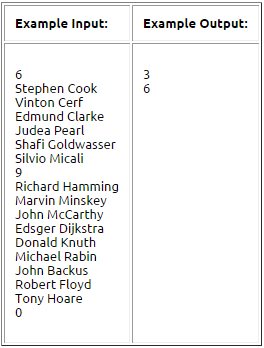
\includegraphics{./src/konigSample.png}
  \end{center}
Entonces la solución sería, utilizando $MaxFlow$:\\
  \source{src/konigSampleCode.cpp}
\section{Teoría de números}
  \subsection{Números romanos}
    A continuación están las funciones para pasar del sistema romano a árabe.\\
    Valores: I = 1, V = 5, X = 10, L = 50, C = 100, D = 500 y M = 1000;
    \subsubsection{Árabe a Romano}
      OJO: Tener en cuenta que el rango de conversión es 1 - 3999
      \source{src/arabicToRoman.cpp}
    \subsubsection{Romano a Árabe}
      OJO: Tener en cuenta que el rango de conversión es 1 - 3999
      \source{src/romanToArabic.cpp}
    \subsection{Divisores de un número}
      Imprime los divisores de un número (cuidado que no lo hace en orden).\\
      Complejidad: $O(\sqrt{n})$ donde $n$ es el número.\\
      \source{./src/divisors.cpp}

  \subsection{Máximo común divisor y mínimo común múltiplo}
  Para hallar el máximo común divisor entre dos números \verb|a| y \verb|b| ejecutar el comando \verb|__gcd(a, b)|.\\
  Para hallar el mínimo común múltiplo: \quad $ \displaystyle\operatorname{lcm}(a, b) = \frac{|a \cdot b|}{\operatorname{gcd}(a,b)}$

  \subsection{Criba de Eratóstenes}
  Encuentra los primos desde 1 hasta un límite $n$.\\
  \verb|sieve[i]| es falso sí y solo sí i es un número primo.\\
  Complejidad: $O(n)$ donde $n$ es el límite superior.\\
  \source{./src/sieve.cpp}

  \subsection{Factorización prima de un número}
  Halla la factorización prima de un número $a$ positivo. Si $a$ es negativo llamar el algoritmo con $|a|$ y agregarle -1 a la factorización.\\
  Se asume que ya se ha ejecutado el algoritmo para generar los primos hasta al menos $\sqrt{a}$.\\
  El algoritmo genera la lista de primos en orden de menor a mayor.\\
  Utiliza el hecho de que en la factorización prima de $a$ aparece máximo un primo mayor a $\sqrt{a}$.\\
  Complejidad aproximada: $O(\sqrt{a})$\\
  \source{./src/factorization.cpp}

  \subsection{Exponenciación logarítmica}
    \subsubsection{Propiedades de la operación módulo}
    \begin{itemize}
      \item $(a \operatorname{mod} n) \operatorname{mod} n = a \operatorname{mod} n$
      \item $(a + b) \operatorname{mod} n = ((a \operatorname{mod} n) + (b\operatorname{mod} n)) \operatorname{mod} n$
      \item $(a \cdot b) \operatorname{mod} n = ((a \operatorname{mod} n) \cdot (b\operatorname{mod} n)) \operatorname{mod} n$
      \item $\displaystyle\left(\frac{a}{b} \right) \operatorname{mod} n \neq \left(\frac{a \operatorname{mod} n}{b\operatorname{mod} n}\right) \operatorname{mod} n$
    \end{itemize}

    \subsubsection{Big mod}
    Halla rápidamente el valor de $b^{\,p} \operatorname{mod} m$ para $0 \leq b,p,m \leq 2147483647$\\
    Si se cambian los valores por \verb|long long| los límites se cambian por $0 \leq b,p \leq 9223372036854775807$ y $1 \leq m \leq 3037000499$.\\
    Complejidad: $O(\operatorname{log} p)$\\
    \source{./src/bigmod.cpp}

  \subsection{Combinatoria}
    \subsubsection{Coeficientes binomiales}
    Halla el valor de $\binom{n}{k}$ para $0 \leq k \leq n \leq 66$. Para $n > 66$ los valores comienzan a ser muy grandes y no caben en un \verb|long long|.\\
    Complejidad: $O(n^2)$\\
    \source{./src/binomial.cpp}

    \subsubsection{Propiedades de combinatoria}
    \begin{itemize}
      \item El número de permutaciones de $n$ elementos diferentes es $n!$
      \item El número de permutaciones de $n$ elementos donde hay $m_1$ elementos repetidos de tipo 1, $m_2$ elementos repetidos de tipo 2,~\ldots, $m_k$ elementos repetidos de tipo $k$ es $$\frac{n!}{m_1! m_2! \cdots m_k!} $$
      \item El número de permutaciones de $k$ elementos diferentes tomados de un conjunto de $n$ elementos es $$ \frac{n!}{(n-k)!} = k! \binom{n}{k}$$
    \end{itemize}



\section{Programación dinámica}
  \subsection{Longest increasing subsequence}
    Halla la longitud de la subsecuencia creciente más larga que hay en un arreglo (también se puede usar con strings).
    \subsubsection{Orden cuadrático}
      Retorna un \textbf{vector con los elementos} que componen la subsecuencia creciente más larga del arreglo $arr$.\\
      Si se necesita sólo la longitud de la subsecuencia ignorar las líneas que tienen comentado un $*$ y retornar lo que se requiera.\\
      Complejidad: $O(n^2)$ donde $n$ es la longitud de~$arr$.
      \source{src/lisn2.cpp}
    \subsubsection{Orden logarítmico imprimiendo sólo longitud}
      Retorna el \textbf{tamaño} de la longitud de la subsecuencia creciente más larga del arreglo $arr$.\\
      Complejidad: $O(n \log_2 n)$ donde $n$ es la longitud de~$arr$.
      \source{src/lislognlength.cpp}
    \subsubsection{Orden logarítmico imprimiendo la secuencia}
      Retorna un \textbf{vector con los elementos} que componen la subsecuencia creciente más larga del arreglo $arr$.\\
      Complejidad: $O(n \log_2 n)$ donde $n$ es la longitud de~$arr$.
      \source{src/lislognelements.cpp}
  \subsection{Problema de la mochila}
  Halla el valor máximo que se puede obtener al empacar un subconjunto de $n$ objetos en una mochila de tamaño $W$ cuando se conoce el valor y el tamaño de cada objeto.\\
Complejidad: $O(n \times W)$ donde $n$ es el número de objetos y $W$ es la capacidad de la mochila.\\
  \source{./src/knapsack.cpp}
  \subsection{Edit distance}
  Calcula cual es el mínimo costo de convertir de un string $s$ al string $t$, utilizando las operaciones de $reemplazar$, $insertar$ y $borrar$.\\
  Complejidad: $O(n \times m)$ donde $n$ y $m$ son los tamaños de los string.
  \source{./src/editDistance.cpp}
  \subsection{Formas de sumar un número}
  Calcula la cantidad de formas en la que puedo obtener un número $n$ con $k$ sumandos.\\
  Complejidad $O(MAXN^2)$ asumiendo, que la $n$ y la $k$ tienen el mismo límite máximo.\\
  Notar que al inicio del main estamos construyendo la matriz, si no es necesario construirla toda, sino hasta la $n$ y $k$ que me den, entonces lo hago.\\
  \source{./src/waysToAdd.cpp}
  \subsection{Longest Common Substring}
  Permite hallar la subcadena común más larga, estrictamente continua, entre dos strings $s$ y $t$.\\
  El ejemplo actual también tiene el método $backtrack$ que permite reconstruir la solución.
  Complejidad $O(n \times m)$ donde $n$ y $m$ son los tamaños del string.
  \source{./src/longestSubString.cpp}
  \subsection{Longest Common Subsequence}
  Halla la longitud de la máxima subsecuencia (no substring) de dos cadenas $s$ y $t$.\\
  Una subsecuencia de una secuencia $s$ es una secuencia que se puede obtener de $s$ al borrarle algunos de sus elementos (probablemente todos) sin cambiar el orden de los elementos restantes.\\
  El algoritmo también se puede aplicar para vectores de elementos, no sólo para strings.\\
  Complejidad: $O(n \times m)$ donde $n$ es la longitud de $s$ y $m$ es la longitud de $t$.\\
  \source{./src/lcs.cpp}
  \subsection{Shortest Common Supersequence}
  El $Shortest$ $Common$ $Supersequence$ es el string más corto $z$ tal que los strings $s$ y $t$ sean subsecuencias de $z$.\\
  Para hallar esto, simplemente es ejecutar el $Longest$ $Common$ $Subsequence$ entre los strings $s$ y $t$, y el tamaño de la supersecuencia más corta será $(n$ + $m)$ - $lcs(s,$ $t)$, donde $n$ y $m$ son los tamaños de los strings $s$ y $t$ respectivamente.
  \subsection{Maximum subarray (non-adjacent) sum (1D)}
    Dado un arreglo con números positivos, encontrar la máxima suma de una subsecuencia, teniendo en cuenta que los números de dicha secuencia no pueden ser adyacentes. \\
    Por ejemplo \texttt{3 2 7 10} debería retornar 13 (suma de 3 y 10), \texttt{3 2 5 10 7} debería retornar 15 (suma de 3, 5 y 7). \\
    Complejidad: $O(n)$ donde $n$ es el tamaño del arreglo.
    \source{./src/non-adjacent_max_sum.cpp}
  \subsection{Maximum subarray sum (1D) - Kadane's Algorithm}
    Encuentra el subarreglo continuo (que contiene al menos un entero positivo) con la suma más grande. \\
    Complejidad: $O(n)$ donde $n$ es el tamaño del arreglo.
    \source{./src/kadane.cpp}
    \subsubsection{Maximum circular subarray sum}
      Si el arreglo es circular y queremos hallar la suma más grande se hace el siguiente procedimiento:
      \begin{itemize}
        \item Aplicamos $Kadane's$ al arreglo sin modificar, y se almacena como máximo: \texttt{maxi}.
        \item Se itera sobre el arreglo para calcular la suma acumulada \texttt{acc} e invertir los valores del arreglo: \texttt{a\_inv[i] = -a[i]}.
        \item La respuesta es el máximo entre el valor del punto $1$ y la suma acumulada más el resultado de un nuevo llamado al algoritmo con el arreglo invertido: \texttt{max(maxi, acc + kadane(a\_inv))}
      \end{itemize}
  \subsection{Maximum subrectangle sum (2D)}
    Permite hallar el sub-rectángulo de una matriz con la mayor suma, la suma de un rectángulo es la suma de todos sus elementos. Un sub-rectángulo es cualquier sub-arreglo continuo de tamaño $1$ $\times$ $1$ o mayor, localizado dentro del toda la matriz.
    \subsubsection{Naïve solution - $O(n^4)$}
      Complejidad: $O(n^4)$ donde $n$ es el tamaño de un lado de la matriz (asumiendo que son iguales). \\
      Cuidado que puede no pasar con 100. Lo idea sería \texttt{MAXN} $= \sqrt[4]{10^6}$
      \source{./src/maximum2DSum.cpp}
    \subsubsection{Using Kadane's - $O(n^3)$}
      \source{./src/max_2d_sum_kadane.cpp}
  \subsection{Maximum subrectangle sum (3D)}
    Permite hallar la mayor suma en un arreglo 3D.
    Complejidad $O(n^6)$ donde $n$ es el tamaño de uno de los lados del cubo.
    \source{./src/maximum3DSum.cpp}
  \subsection{Partition problem}
    Determina si un arreglo de números puede ser particionado en dos conjuntos tal que la suma de ambos sea la misma. \\
    Complejidad: $O(sum * n)$, donde $n$ es el tamaño del arreglo y $sum$ es la suma de cada conjunto. (notar que este algoritmo no es eficiente para arreglos con grandes sumas, para ese caso intentar una solución recursiva $O(2^n)$)
    \source{./src/partition_problem.cpp}
  \subsection{Longest Palindromic Substring}
    Dado un string, encontrar el substring (estrictamente continuo) más largo que sea palíndromo. Por ejemplo si tenemos \texttt{"forgeeksskeegfor"} la salida debería ser: \texttt{"geeksskeeg"}\\
    Complejidad: Creo que el primer método $O(n^3)$, el segundo $O(n)$ y el tercero $O(n^2)$.
    \source{./src/longest_palindromic_substring.java}
  \subsection{Longest Palindromic Subsequence}
    Dado un string, encontrar el tamaño de la subsecuencia (no necesariamente continua). Por ejemplo  para \texttt{BBABCBCAB} la respuesta es 7, porque \texttt{BABCBAB} es la subsecuencia palindrómica más larga.
    \source{./src/longest_palindromic_subsequence.cpp}
  \subsection{Text Justification}
    Dada una secuencia de palabras y un número límite de caracteres
    que pueden escribirse en una línea, poner los fin de líneas en la
    secuencia dada tal que las líneas queden impresas equitativamente
    (En cuanto espacios en blanco)
    Complejidad: $O(n^2)$.
    \source{./src/text_justification.java}

\section{Geometría}
  \subsection{Closest pair of points in a plane}
    Finds the smallest distance from a given set of points.
    \source{./src/closest_pair_points.cpp}

\section{Strings}
  \subsection{Algoritmo de KMP}
    Encuentra si el string \verb|needle| aparece en en string \verb|haystack|.\\
    Si no se retorna directamente \verb|true| cuando se halla la primera ocurrencia, el algoritmo encuentra todas las ocurrencias de \verb|needle| en \verb|haystack|.\\
    La primera parte del algoritmo llena el arreglo \verb|border| donde \verb|border[i]| es la longitud del borde del prefijo de \verb|needle| que termina en la posición \verb|i|. Un borde de una cadena $s$ es la cadena más larga que es a la vez prefijo y sufijo de $s$ pero que es diferente de $s$.\\
    Complejidad: $O(n)$ donde $n$ es el tamaño de \verb|haystack|.\\
    \source{./src/kmp.cpp}

  \subsection{Algoritmo de Booth - Lexicographically minimal string rotation}
    Encuentra la rotación de un string que contiene el menor orden lexicográfico de todas las rotaciones posibles. Por ejemplo, la menor rotación lexicográfica de \texttt{bbaaccaadd} sería \texttt{aaccaaddbb}, y de \texttt{abcdeabcdea} sería \texttt{aabcdeabcde}. \\
    El algoritmo concatena el string a sí mismo y computa una tabla basándose en el algoritmo de KMP.\\
    El método devuelve el \textbf{índice en base 0 a primera letra correspondiente a la mejor rotación}, si se necesita el string completo se deberá utilizar substring para reconstruirlo: \texttt{str.substr(ind, str.size()) + str.substr(0, ind)}\\
Complejidad: $O(n)$ donde $n$ es el tamaño del string.
    \source{./src/booths.cpp}

  \subsection{Formatos de impresión}
    \subsubsection{Números}
    Con la función $printf$ podemos dar distintos formatos de impresión, por ejemplo justificar, ceros o espacios iniciales, etc.
      \source{./src/printFormat.cpp}
    \subsubsection{Strings}
    \begin{itemize}
      \item The printf(“\%s", “Hello, world!”); statement prints the string (nothing special happens.)
      \item The printf(“\%15s", “Hello, world!”); statement prints the string, but print 15 characters. If the string is smaller the “empty” positions will be filled with “whitespace.”
      \item The printf(“\%.10s”, “Hello, world!”); statement prints the string, but print only 10 characters of the string.
      \item The printf(“\%-10s”, “Hello, world!”); statement prints the string, but prints at least 10 characters. If the string is smaller “whitespace” is added at the end. (See next example.)
      \item The printf(“\%-15s”, “Hello, world!”); statement prints the string, but prints at least 15 characters. The string in this case is shorter than the defined 15 character, thus “whitespace” is added at the end (defined by the minus sign.)
      \item The printf(“\%.15s”, “Hello, world!”); statement prints the string, but print only 15 characters of the string. In this case the string is shorter than 15, thus the whole string is printed.
      \item The printf(“\%15.10s”, “Hello, world!”); statement prints the string, but print 15 characters.
If the string is smaller the “empty” positions will be filled with “whitespace.” But it will only print a maximum of 10 characters, thus only part of new string (old string plus the whitespace positions) is printed.
      \item The printf(“\%-15.10s”, “Hello, world!”); statement prints the string, but it does the exact same thing as the previous statement, accept the “whitespace” is added at the end.
    \end{itemize}
    \subsubsection{Formato en Java}
    Para utilizar formatos de impresión en Java se debe usar $System.out.format$ y darle formatos muy parecidos a los de C++, acá podemos ver varios ejemplos. Se pueden dar incluso formatos para impresión de $Calendar$.
    \source{./src/printFormatJava.java}

\section{Otros}
  \subsection{Binary Search}
    Permite buscar un elemento ($key$) en un arreglo \textbf{ordenado} ($arr$).
    Complejidad: $O(n \log_2 n)$ donde $n$ es la cantidad de elementos del arreglo.\\
    \source{./src/binarySearch.cpp}
    \subsubsection{Traditional algorithm}
      Returns the index of some element that is equal to the given value (if there are multiple
      elements, it returns some arbitrary one).
      \source{./src/binary_search.cpp}
    \subsubsection{Lower bound}
      Returns the leftmost place where the given element can be correctly inserted.
      \source{./src/lower_bound.cpp}
    \subsubsection{Upper bound}
      Returns the rightmost place where the given element can be correctly inserted.
      \source{./src/upper_bound.cpp}
  \subsection{Binary Search Tree (BST)}
    \subsubsection{Largest BST in a Binary Tree}
      Dado un árbol binario, encontrar el tamaño del BST más grande en ese árbol.
      \source{./src/largest_bst.java}
  \subsection{Build Binary Tree from PreOrder and InOrder}
    Permite crear un Binary Tree partiendo de los valores de PreOrden e InOrder del BT, el resultado sera un String con el posOrder del BT.
    \source{./src/build-BT-from-pre-in.cpp}
  \subsection{BitSet}
    Almacena bits, simula un array de booleanos, optimizando el espacio, cada elemento puede ser accedido por el operador $[$ $]$\\
    \source{./src/bitset.cpp}
  \subsection{Máximo orden dado un $n$}
    En la siguiente tabla se encuentran los límites de orden máximo respecto a un número de elementos $n$ del problema.\\
    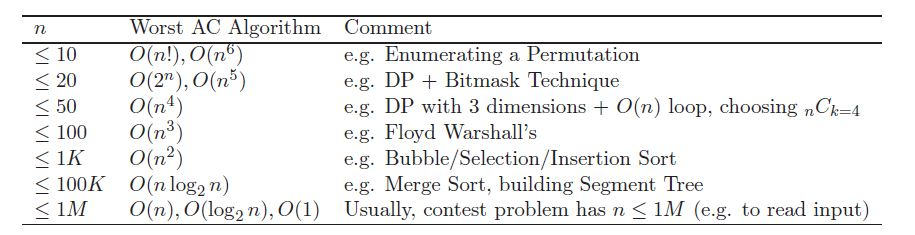
\includegraphics[scale=0.5]{./src/maxorder.jpg}
  \subsection{Suma de grandes números en C++}
    Como sabemos, en C++ los enteros ($int$) tienen un rango de $(2^31)-1$, y los $long long$ tienen un rango de $(2^64)-1$, por esto no podemos almacenar números de más de 18~19 números, para esto se debe usar la clase $BigInteger$ en $Java$, o si no hay que preocuparse por tiempo, podemos representar los números como $string$ y utilizar la siguiente funciones como la siguiente:
    \source{./src/bigIntegerCpp.cpp}
  \subsection{Largest Rectangle in a Histogram}
    Encuentra el área rectangular más grande posible en un histograma, donde el rectángulo es determinado por un número de barras continuas. Se asume que todas las barras tienen el mismo ancho de 1 unidad. \\
    Complejidad: $O(n)$ donde $n$ es la cantidad de barras en el histograma.
    \source{./src/largest_rectangle.cpp}

\section{Struct}
  Las estructuras en C++ son muy útiles a la hora de hacer algún tipo de dato muy específico o usar funciones de comparación personalizadas
  \subsection{Función de comparación}
  En este caso tenemos una función de comparación que involucra los dos atributos $x$ y $y$ de la estructura $dato$
  \source{./src/struct.cpp}
  \subsection{Radix sort}
  Complejidad: $O(w \times n)$ donde $n$ es la cantidad de elementos del arreglo y $w$ la longitud del mayor número.\\
  \source{./src/radixSort.cpp}

\section{C++}
  \subsection{Strings con arreglo de caracteres}
  Para lograr una implementación eficiente, se pueden trabajar los strings como arreglo de caracteres, es decir, como en C, existen varias funciones que pueden ser útiles, NOTA: no todas las funciones se encuentran en el ejemplo.
  \source{./src/getsScanfGetline.cpp}


\end{document}
